\documentclass[12pt,a4paper,twoside]{report}
% -------------------------------------------------------------------- %
% Pacotes

\usepackage[utf8]{inputenc}
\usepackage[T1]{fontenc}
\usepackage[brazil]{babel}
\usepackage[fixlanguage]{babelbib}
\usepackage[pdftex]{graphicx}      % usamos arquivos pdf/png como figuras
\usepackage{setspace}              % espaçamento flexvel
\usepackage{indentfirst}           % indentação do primeiro parágrafo
\usepackage{makeidx}               % índice remissivo
\usepackage[nottoc]{tocbibind}     % acrescentamos a bibliografia/indice/conteudo no Table of Contents
\usepackage{courier}               % usa o Adobe Courier no lugar de Computer Modern Typewriter
\usepackage{type1cm}               % fontes realmente escaláveis
\usepackage{titletoc}
\usepackage{ucs}
\usepackage[font=small,format=plain,labelfont=bf,up,textfont=it,up]{caption}
\usepackage[usenames,svgnames,dvipsnames]{xcolor}
\usepackage[a4paper,top=2.54cm,bottom=2.0cm,left=2.0cm,right=2.54cm]{geometry} % margens
\usepackage{amsmath}
\usepackage{booktabs} % cria tabelas em formato profissional
\usepackage[pdftex,plainpages=false,pdfpagelabels,pagebackref,colorlinks=true,citecolor=DarkGreen,
linkcolor=NavyBlue,urlcolor=DarkRed,filecolor=green,bookmarksopen=true]{hyperref} % links coloridos
\usepackage[all]{hypcap}                % soluciona o problema com o hyperref e capítulos
\usepackage[square,sort,nonamebreak,comma]{natbib}  % citação bibliográfica alpha
\fontsize{60}{62}\usefont{OT1}{cmr}{m}{n}{\selectfont}
\usepackage{upquote}                    % formata apóstrofes '
\usepackage{textcomp}

% Para formatar corretamente as URLs
\usepackage{url}
% -------------------------------------------------------------------- %
% Cabeçalhos similares ao TAOCP de Donald E. Knuth
\usepackage{fancyhdr}
\pagestyle{fancy}
\fancyhf{}
\renewcommand{\chaptermark}[1]{\markboth{\MakeUppercase{#1}}{}}
\renewcommand{\sectionmark}[1]{\markright{\MakeUppercase{#1}}{}}
\renewcommand{\headrulewidth}{0pt}

\frenchspacing                     % arruma o espaço: id est (i.e.) e exempli gratia (e.g.)
\urlstyle{same}                    % URL com o mesmo estilo do texto e no mono-spaced
\makeindex                         % para o índice remissivo
\raggedbottom                      % para no permitir espaços extras no texto
\fontsize{60}{62}\usefont{OT1}{cmr}{m}{n}{\selectfont}
\cleardoublepage
\normalsize

% -------------------------------------------------------------------- %
% Cores para formatação de código
\usepackage{color}
\definecolor{vermelho}{rgb}{0.6,0,0} % para strings
\definecolor{verde}{rgb}{0.25,0.5,0.35} % para comentários
\definecolor{roxo}{rgb}{0.5,0,0.35} % para palavras-chaves
\definecolor{azul}{rgb}{0.25,0.35,0.75} % para strings
\definecolor{cinza-claro}{gray}{0.95}
% -------------------------------------------------------------------- %
% Opções de listagem usados para o código fonte
% Ref: http://en.wikibooks.org/wiki/LaTeX/Packages/Listings
\usepackage{listings}           % para formatar código-fonte (ex. em Java)

\lstset{ %
language=Python,                      % seleciona a linguagem do código
basicstyle=\footnotesize\ttfamily,    % o tamanho da fonte usado no código
commentstyle=\color{verde}\bfseries,  % formatação de comentários
stringstyle=\color{azul},             % formatação de strings
upquote=true,
numbers=left,                   % onde colocar os números de linha
numberstyle=\tiny,  % o tamanho da fonte usada para a numeração das linhas
stepnumber=1,                   % o intervalo entre dois números de linhas. Se for 1, numera cada uma.
numbersep=5pt,                  % how far the line-numbers are from the code
showspaces=false,               % show spaces adding particular underscores
showstringspaces=false,         % underline spaces within strings
showtabs=false,                 % show tabs within strings adding particular underscores
keywordstyle=\color{roxo}\bfseries,
keywordstyle=[1]\color{roxo}\bfseries,
keywordstyle=[2]\color{verde}\bfseries,
frame=b,                   % adds a frame around the code
framerule=0.6pt,
tabsize=2,                      % sets default tabsize to 2 spaces
captionpos=t,                   % sets the caption-position to top
breaklines=true,                % sets automatic line breaking
breakatwhitespace=false,        % sets if automatic breaks should only happen at whitespace
escapeinside={\%*}{*)},         % if you want to add a comment within your code
backgroundcolor=\color[rgb]{1.0,1.0,1.0}, % choose the background color.
rulecolor=\color[rgb]{0.8,0.8,0.8},
extendedchars=true,
xleftmargin=10pt,
xrightmargin=10pt,
framexleftmargin=10pt,
framexrightmargin=10pt,
literate={â}{{\^{a}}}1  % para formatar corretamente os acentos do Português ao usar utf8
    {ê}{{\^{e}}}1
    {ô}{{\^{o}}}1
    {Â}{{\^{A}}}1
    {Ê}{{\^{E}}}1
    {Ô}{{\^{O}}}1
    {á}{{\'{a}}}1
    {é}{{\'{e}}}1
    {í}{{\'{i}}}1
    {ó}{{\'{o}}}1
    {ú}{{\'{u}}}1
    {Á}{{\'{A}}}1
    {É}{{\'{E}}}1
    {Í}{{\'{I}}}1
    {Ó}{{\'{O}}}1
    {Ú}{{\'{U}}}1
    {à}{{\`{a}}}1
    {À}{{\`{A}}}1
    {ã}{{\~{a}}}1
    {õ}{{\~{o}}}1
    {Ã}{{\~{A}}}1
    {Õ}{{\~{O}}}1
    {ç}{{\c{c}}}1
    {Ç}{{\c{C}}}1
    {ü}{{\"u}}1
    {Ü}{{\"U}}1
}

\renewcommand{\lstlistingname}{Listagem}
\renewcommand{\lstlistlistingname}{Lista de Listagens}

% \captionsetup[lstlisting]{singlelinecheck=false, labelfont={blue}, textfont={blue}}
\usepackage{caption}
\DeclareCaptionFont{white}{\color{white}}
\DeclareCaptionFormat{listing}{\colorbox[cmyk]{0.43, 0.35, 0.35,0.01}{\parbox{\textwidth}{\hspace{15pt}#1#2#3}}}
\captionsetup[lstlisting]{format=listing,labelfont=white,textfont=white, singlelinecheck=false, margin=0pt, font={bf,footnotesize}}

\title{Análise experimental de algoritmos usando Python}
\author{Patricia Mariana Ramos Marcolino \\
\texttt{\small \url{pnrmarcolino@hotmail.com}}
\vspace{1cm} \\
Eduardo Pinheiro Barbosa \\
\texttt{\small \url{eduardptu@homail.com}}
\vspace{1cm} \\
Faculdade de Computação \\
Universidade Federal de Uberlândia
}
\date{\today}

\begin{document}
\maketitle
% -------------------------------------------------------------------- %
% Listas de figuras, tabelas e códigos criadas automaticamente
\listoffigures
\listoftables
\lstlistoflistings
% -------------------------------------------------------------------- %

% -------------------------------------------------------------------- %
% Sumário
\tableofcontents
% cabeçalho para as páginas de todos os capítulos
\fancyhead[RE,LO]{\thesection}

%\singlespacing              % espaçamento simples
\setlength{\parskip}{0.15in} % espaçamento entre paragráfos

\chapter{Análise}

A relação de recorrência que expressa a complexidade de tempo do insertion-sort é: $T(n) = T(n - 1) + n $
Essa relação nos diz que o tempo do {\it insertion-sort} é igual ao tempo que a hipótese de indução gasta para ordenar os $n - 1$ elementos, mais o tempo gasto para inserir um elemento na sequência ordenada.
Resolvendo a recorrência temos:

\[T(n) = T(n - 1) + n\]
\[ = T(n - 2) + (n -1) + n\]
\[T(n) = T(n - 3) + (n - 2) + (n - 1) + n\]
\[...\]
\[T(n) = T(1) + 2 + 3 + 4 + 5 + ... + (n - 1) + n\]
\[T(n) = n(n + 1)/2\]
\[T(n) = O(n^2)\]

Ou seja, a complexidade de tempo do {\it insertion-sort} é limitada pela função quadrática.


\chapter{Resultados}
\section{Tabelas}

\input{../insertionsort/tabelas/insertionsortAleatorio.tex}

\begin{figure}[ht]
\centering 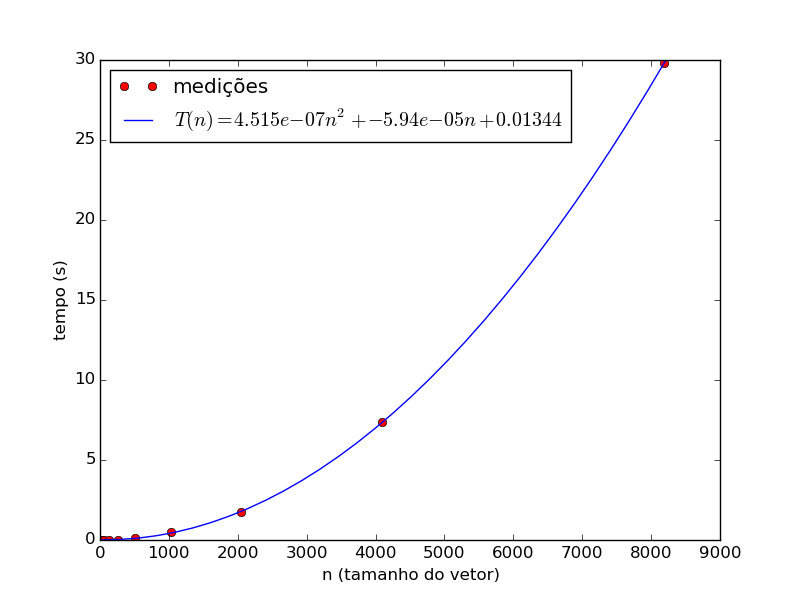
\includegraphics[scale=0.8]{../insertionsort/imagens/insertionsortAleatorio0.png}
\caption{A análise do grafico para $2^{32}$ segue abaixo para insertionsort de vetor aleatório.\\
Tendo a função $T(n) = 4.515\mathrm{e}-07*n^2+5.94\mathrm{e}0.5*n-0.013344$ e para o $n =2^{32}$, $T(2^{32}) = 8.11658 * 10^{301}$}
\label{fig:bolhaAleatorio0}
\end{figure}

\begin{figure}[ht]
\centering 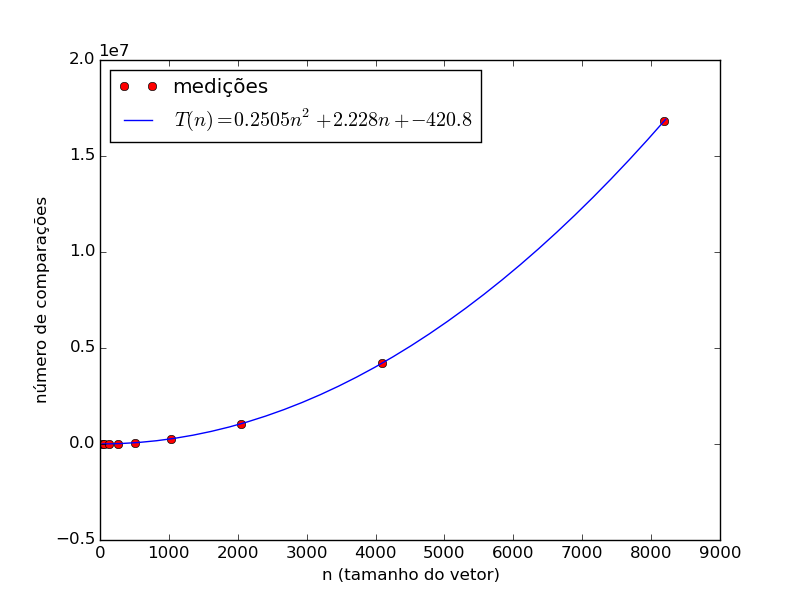
\includegraphics[scale=0.8]{../insertionsort/imagens/insertionsortAleatorio1.png}
\caption{A análise em número de comparações do grafico para $2^{32}$ segue abaixo para bobblesort de vetor aleatório.\\
Tendo a função $T(n) = 0.2505*n^2 + 2.228*n - 420.8$ e para o $n =2^{32}$, $T(2^{32}) = 4.5032213 * 10^{307}$}
\label{fig:bolhaAleatorio1}
\end{figure}


\input{../insertionsort/tabelas/insertionsortCrescente.tex}

\begin{figure}[ht]
\centering 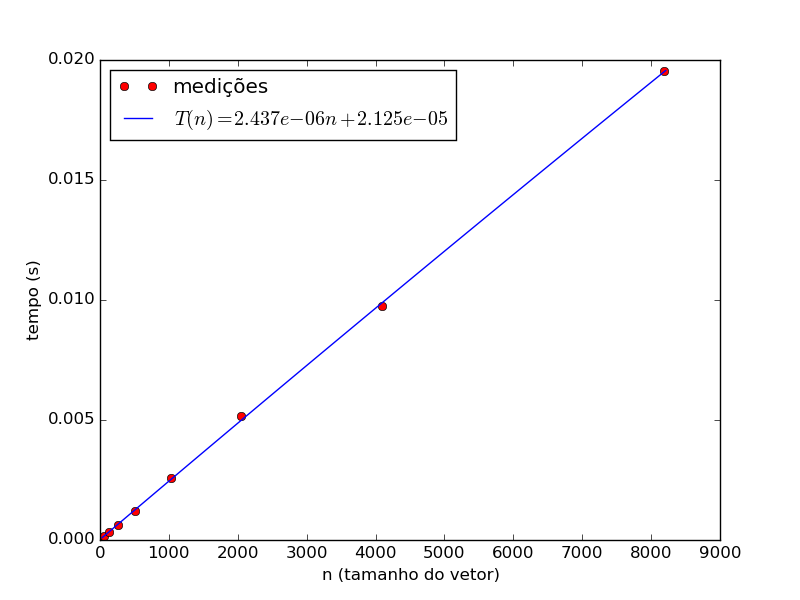
\includegraphics[scale=0.8]{../insertionsort/imagens/insertionsortCrescente0.png}
\caption{A análise do grafico para $2^{32}$ segue abaixo para insertionsort de vetor crescente.\\
Tendo a função $T(n) = 2.437\mathrm{e}-06*n+1.125\mathrm{e}-05$ e para o $n =2^{32}$, $T(2^{32}) = 10466.835311602$}
\label{fig:insertionsortCrescente0}
\end{figure}

\begin{figure}[ht]
\centering 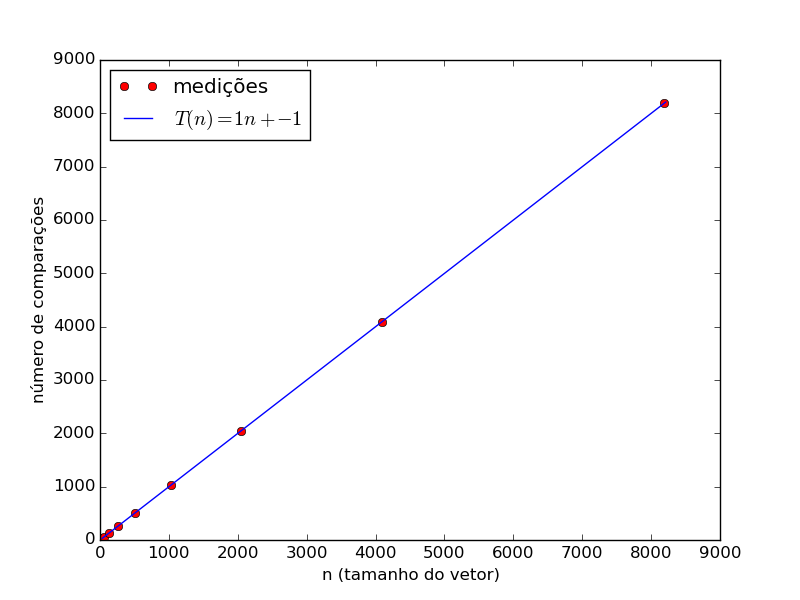
\includegraphics[scale=0.8]{../insertionsort/imagens/insertionsortCrescente1.png}
\caption{A análise em número de comparações do grafico para $2^{32}$ segue abaixo para bobblesort de vetor crescente.\\
Tendo a função $T(n) = 1*n - 1$ e para o $n =2^{32}$, $T(2^{32}) = 4294967295$}
\label{fig:insertionsortCrescente1}
\end{figure}


\input{../insertionsort/tabelas/insertionsortDecrescente.tex}

\begin{figure}[ht]
\centering 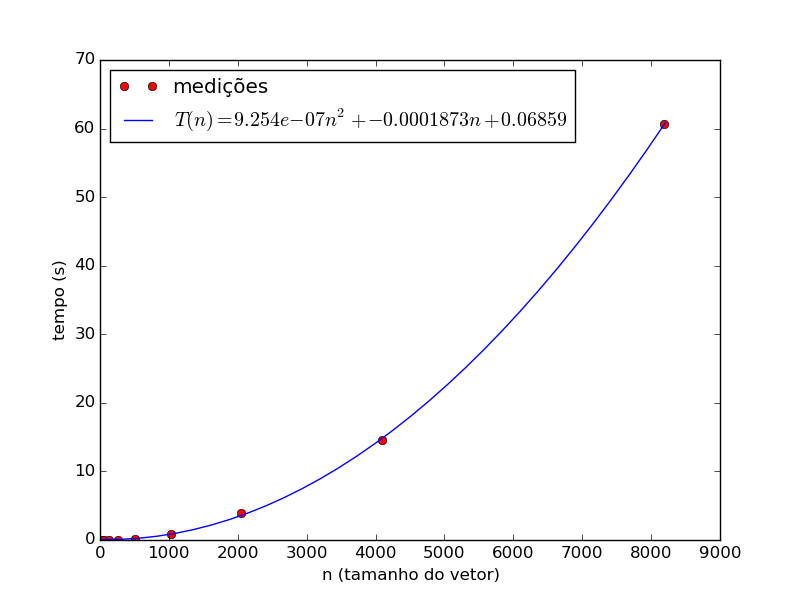
\includegraphics[scale=0.8]{../insertionsort/imagens/insertionsortDecrescente0.png}
\caption{A análise do grafico para $2^{32}$ segue abaixo para insertionsort de vetor decrescente.\\
Tendo a função $T(n) = 9.254\mathrm{e}-07*n^2-0.0001873*n+0.06859$ e para o $n =2^{32}$, $T(2^{32}) = 1.66358522 * 10^{302}$}
\end{figure}

\begin{figure}[ht]
\centering 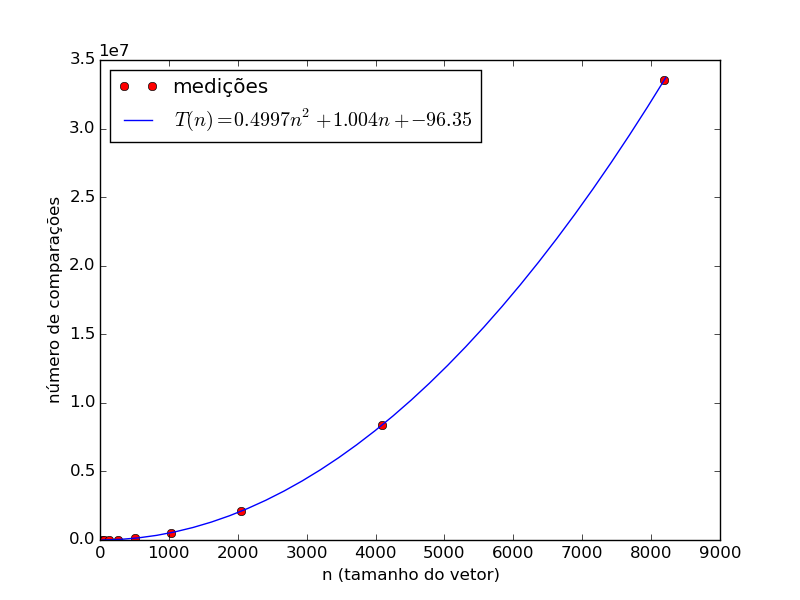
\includegraphics[scale=0.8]{../insertionsort/imagens/insertionsortDecrescente1.png}
\caption{A análise do grafico para $2^{32}$ segue abaixo para insertionsort de vetor decrescente.\\
Tendo a função $T(n) = 0.4997*n^2+1.004*n-96.35$ e para o $n =2^{32}$, $T(2^{32}) = 8.98307259 * 10^{307}$}
\label{fig:insertionsortDecrescente1}
\end{figure}


\input{../insertionsort/tabelas/insertionsortQuaseCresc10.tex}

\begin{figure}[ht]
\centering 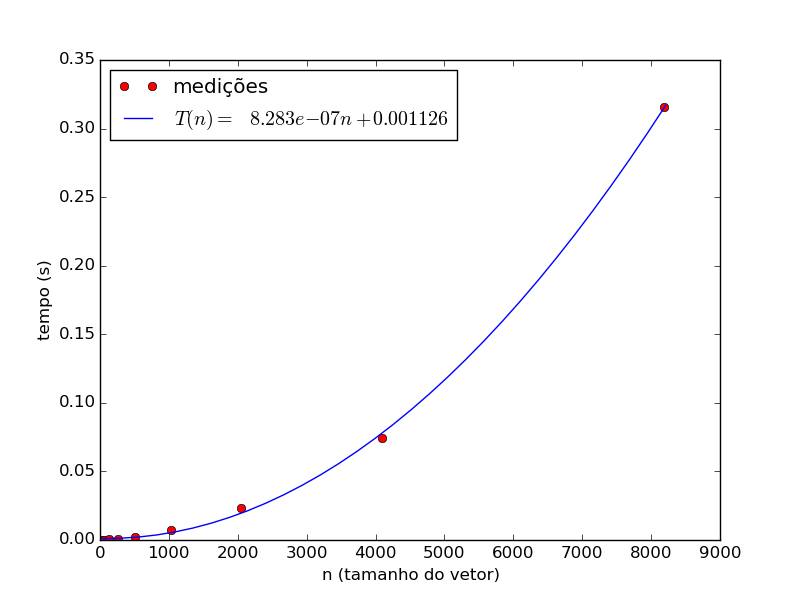
\includegraphics[scale=0.8]{../insertionsort/imagens/insertionsortQuaseCresc100.png}
\caption{A análise do grafico para $2^{32}$ segue abaixo para insertionsort de vetor quase crescente 10\%.\\
Tendo a função $T(n) = 8.283\mathrm{e}-07*n^2 - 7*n+0.001126$ e para o $n =2^{32}$, $T(2^{32}) =1.4890*10^302 $}
\label{fig:insertionsortQuaseCresc100}
\end{figure}

\begin{figure}[ht]
\centering 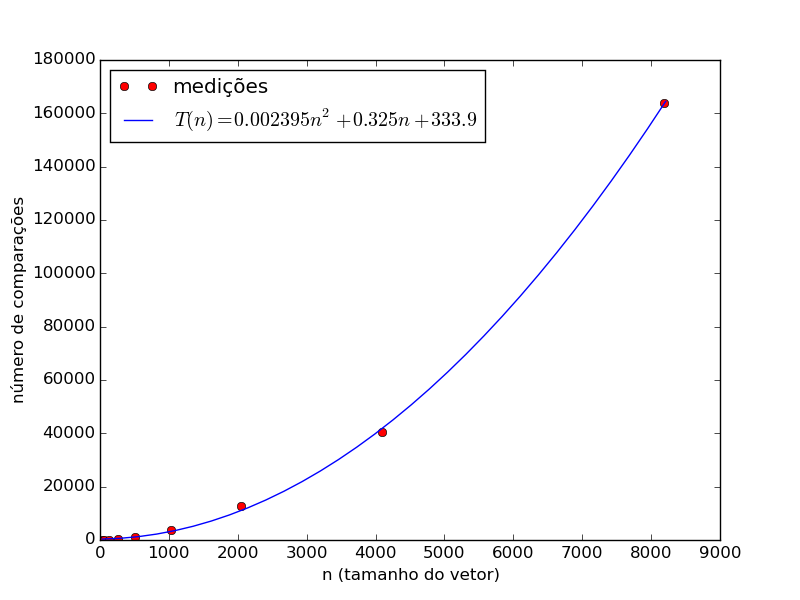
\includegraphics[scale=0.8]{../insertionsort/imagens/insertionsortQuaseCresc101.png}
\caption{A análise do grafico para $2^{32}$ segue abaixo para insertionsort de vetor quase crescente 10\%.\\
Tendo a função $T(n) = 0.002395*n^2+0.325*n+333.9$ e para o $n =2^{32}$, $T(2^{32}) 4.30547505 * 10^{305}$}
\label{fig:insertionsortQuaseCresc101}
\end{figure}


\begin{table}[ht]
\centering
\begin{tabular}{rrr} \toprule
        n &    comparações &       tempo(s) \\ \midrule
      32  &             40 &      0.000092 \\
      64  &            103 &      0.000233 \\
     128  &            277 &      0.000577 \\
     256  &            853 &      0.001586 \\
     512  &           2635 &      0.004985 \\
    1024  &          11369 &      0.019259 \\
    2048  &          37524 &      0.067758 \\
    4096  &         155991 &      0.285469 \\
    8192  &         618930 &      1.055770 \\
\bottomrule\addlinespace
\end{tabular}
\caption{Tabela com vetor teste quase crescente 20\%: a linha de interesse analisada para este caso é a 15}
\label{tab:insertionsortQuaseCresc20}
\end{table}


\begin{figure}[ht]
\centering 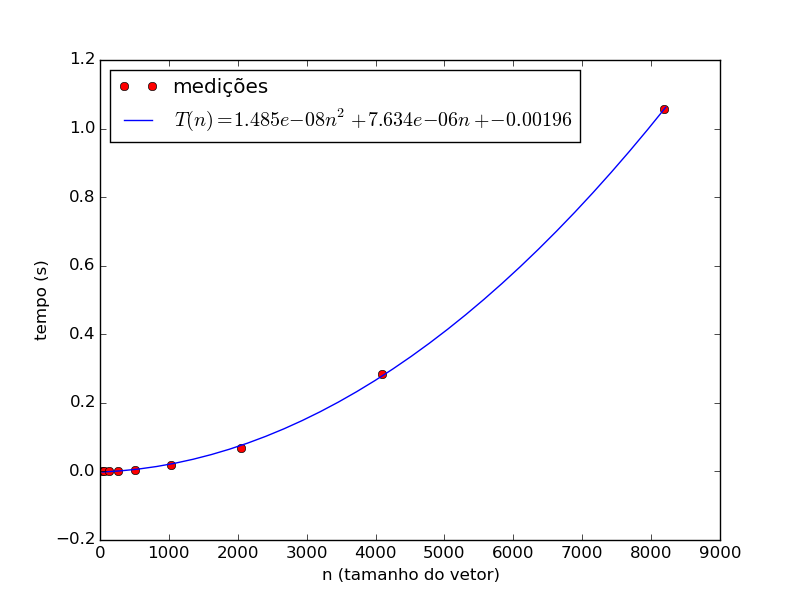
\includegraphics[scale=0.8]{../insertionsort/imagens/insertionsortQuaseCresc200.png}
\caption{A análise do grafico para $2^{32}$ segue abaixo para insertionsort de vetor quase crescente 20\%.\\
Tendo a função $T(n) = 1.485\mathrm{e}-08*n^2+7.634\mathrm{e}-06n -0.00196$ e para o $n =2^{32}$, $T(2^{32}) = 2.66957430 * 10^{300}$}
\label{fig:insertionsortQuaseCresc200}
\end{figure}

\begin{figure}[ht]
\centering 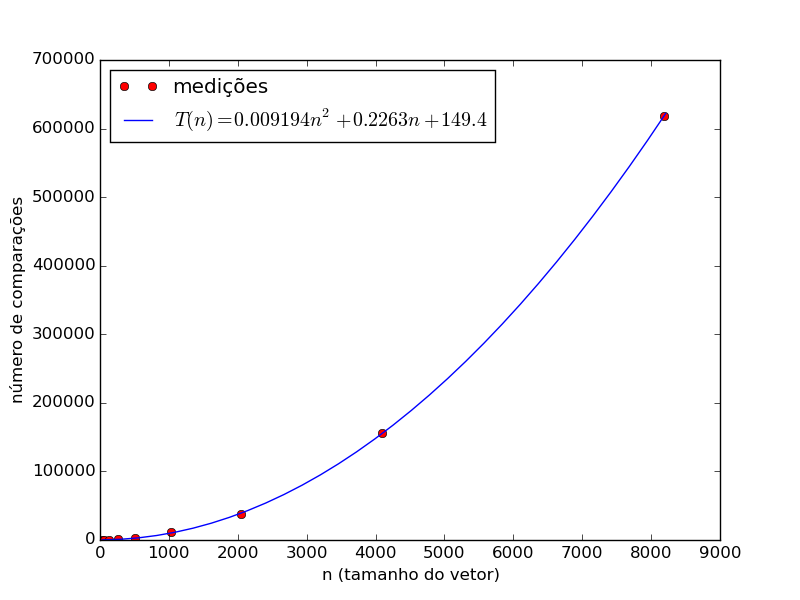
\includegraphics[scale=0.8]{../insertionsort/imagens/insertionsortQuaseCresc201.png}
\caption{A análise do grafico para $2^{32}$ segue abaixo para insertionsort de vetor quase crescente 20\%.\\
Tendo a função $T(n) = 0.009194*n^2+0.2263*n+149.4$ e para o $n =2^{32}$, $T(2^{32}) = 1.6527990 * 10^{306}$}
\label{fig:insertionsortQuaseCresc201}
\end{figure}

\clearpage
\begin{table}[ht]
\centering
\begin{tabular}{rrr} \toprule
        n &    comparações &       tempo(s) \\ \midrule
      32  &             44 &      0.000110 \\
      64  &            145 &      0.000296 \\
     128  &            505 &      0.000954 \\
     256  &           1352 &      0.002361 \\
     512  &           6396 &      0.010923 \\
    1024  &          23767 &      0.043876 \\
    2048  &          91546 &      0.162196 \\
    4096  &         341389 &      0.555987 \\
    8192  &        1390938 &      2.385560 \\
\bottomrule\addlinespace
\end{tabular}
\caption{Tabela com vetor teste quase crescente 30\%: a linha de interesse analisada para este caso é a 15}
\label{tab:insertionsortQuaseCresc30}
\end{table}


\begin{figure}[ht]
\centering 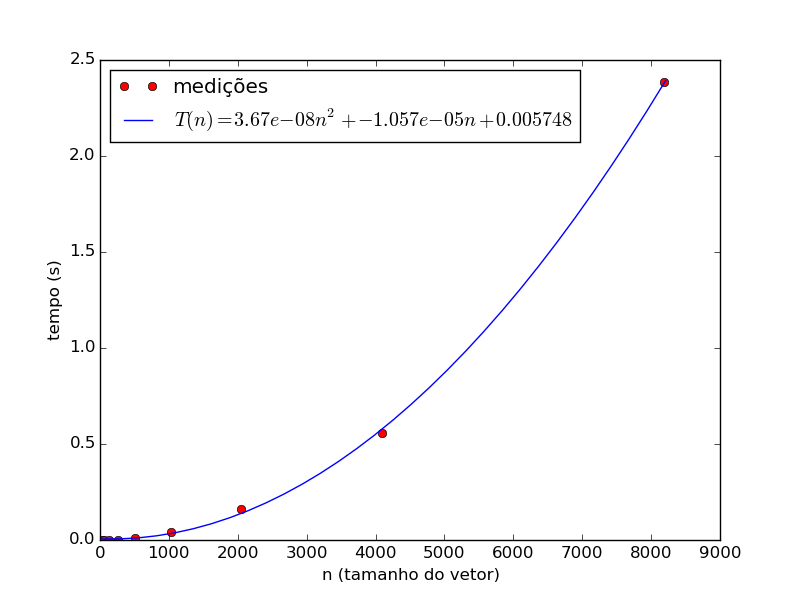
\includegraphics[scale=0.8]{../insertionsort/imagens/insertionsortQuaseCresc300.png}
\caption{A análise do grafico para $2^{32}$ segue abaixo para insertionsort de vetor quase crescente 30\%.\\
Tendo a função $T(n) = 3.67\mathrm{e}-08*n^2+1.057\mathrm{e}-05*n+0.005748$ e para o $n =2^{32}$, $T(2^{32}) = 6.59753380 * 10^{300}$}
\label{fig:insertionsortQuaseCresc300}
\end{figure}

\begin{figure}[ht]
\centering 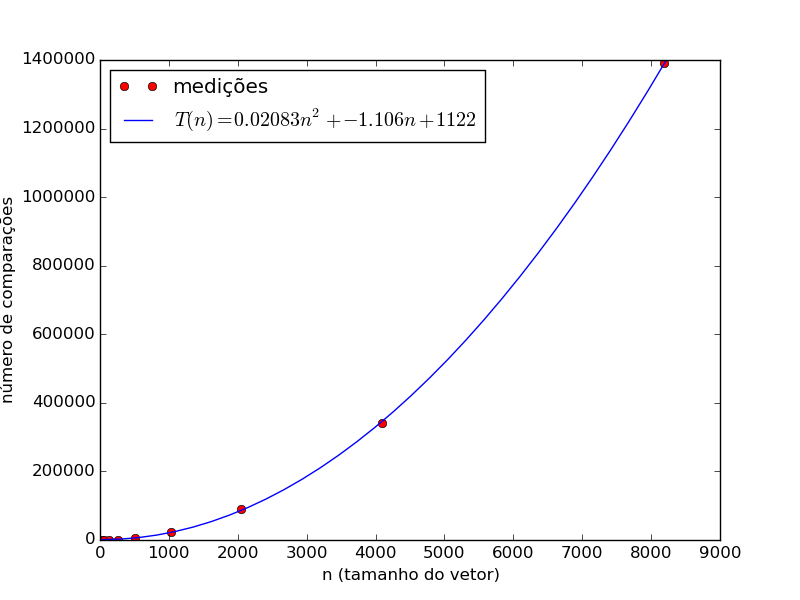
\includegraphics[scale=0.8]{../insertionsort/imagens/insertionsortQuaseCresc301.png}
\caption{A análise do grafico para $2^{32}$ segue abaixo para insertionsort de vetor quase crescente 30\%.\\
Tendo a função $T(n) = 0.02083*n^2+1.106*n+1122$ e para o $n =2^{32}$, $T(2^{32}) = 3.744594 * 10^{306}$}
\label{fig:insertionsortQuaseCresc301}
\end{figure}


\input{../insertionsort/tabelas/insertionsortQuaseCresc40.tex}

\begin{figure}[ht]
\centering 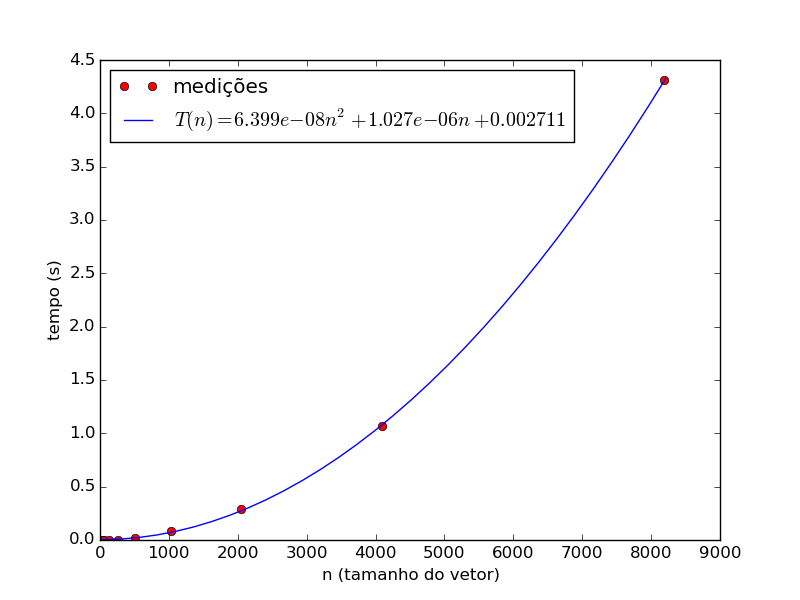
\includegraphics[scale=0.8]{../insertionsort/imagens/insertionsortQuaseCresc400.png}
\caption{A análise do grafico para $2^{32}$ segue abaixo para insertionsort de vetor quase crescente 40\%.\\
Tendo a função $T(n) = 6.399\mathrm{e}-08*n^2+1.027\mathrm{e}-06*n+0.002711$ e para o $n =2^{32}$, $T(2^{32}) = 1.15034383 * 10^{301}$}
\label{fig:insertionsortQuaseCresc400}
\end{figure}

\begin{figure}[ht]
\centering 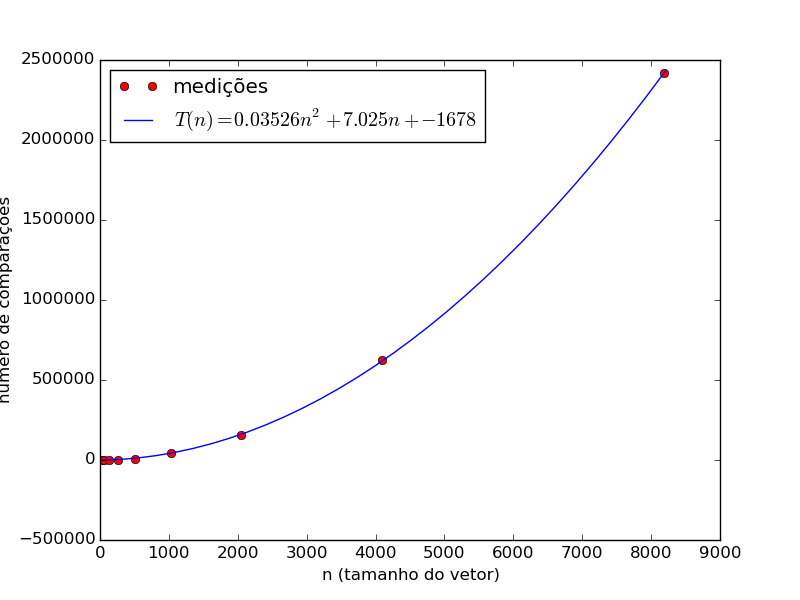
\includegraphics[scale=0.8]{../insertionsort/imagens/insertionsortQuaseCresc401.png}
\caption{A análise do grafico para $2^{32}$ segue abaixo para insertionsort de vetor quase crescente 40\%.\\
Tendo a função $T(n) = 0.03526*n^2+7.025*n+1678$ e para o $n =2^{32}$, $T(2^{32}) = 6.33866599 * 10^{306}$}
\label{fig:insertionsortQuaseCresc401}
\end{figure}


\input{../insertionsort/tabelas/insertionsortQuaseCresc50.tex}

\begin{figure}[ht]
\centering 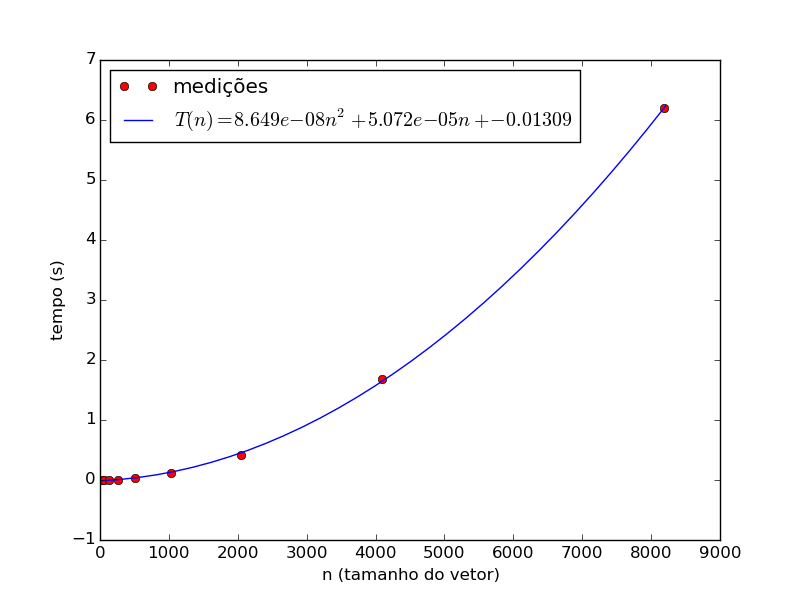
\includegraphics[scale=0.8]{../insertionsort/imagens/insertionsortQuaseCresc500.png}
\caption{A análise do grafico para $2^{32}$ segue abaixo para insertionsort de vetor quase crescente 50 \%.\\
Tendo a função $T(n) = 8.649\mathrm{e}-08*n^2+5.07\mathrm{e}*n-05-0.01309$ e para o $n =2^{32}$, $T(2^{32}) = 1.55482 * 10^{301}$}
\label{fig:insertionsortQuaseCresc500}
\end{figure}

\begin{figure}[ht]
\centering 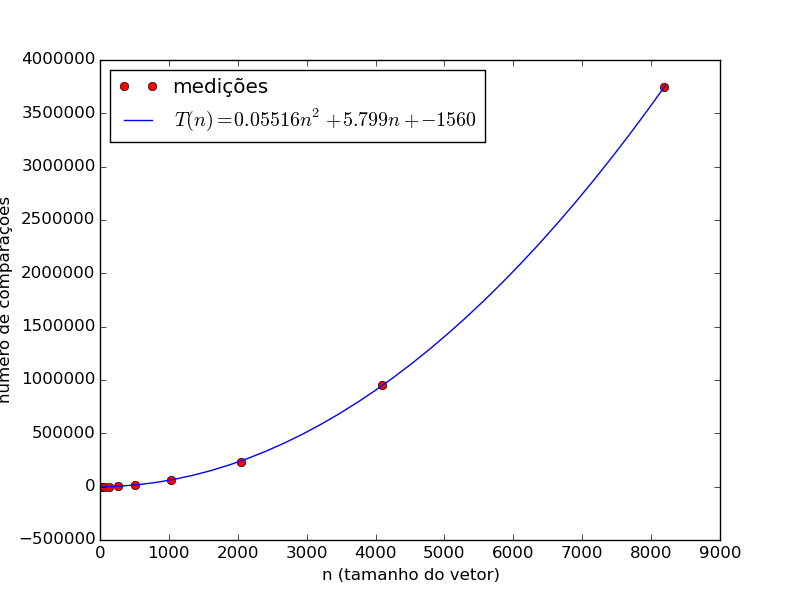
\includegraphics[scale=0.8]{../insertionsort/imagens/insertionsortQuaseCresc501.png}
\caption{A análise do grafico para $2^{32}$ segue abaixo para insertionsort de vetor quase crescente 50\%.\\
Tendo a função $T(n) = 0.05516*n^2+5799*n-1560$ e para o $n =2^{32}$, $T(2^{32}) = 9.9160753 * 10^{306}$}
\label{fig:insertionsortQuaseCresc501}
\end{figure}


\begin{table}[ht]
\centering
\begin{tabular}{rrr} \toprule
        n &    comparações &       tempo(s) \\ \midrule
      32  &            524 &      0.000919 \\
      64  &           2073 &      0.003547 \\
     128  &           8208 &      0.013749 \\
     256  &          32731 &      0.057140 \\
     512  &         130747 &      0.213553 \\
    1024  &         522102 &      0.972133 \\
    2048  &        2088710 &      3.766950 \\
    4096  &        8351700 &     14.581000 \\
    8192  &       33395428 &     56.434800 \\
\bottomrule\addlinespace
\end{tabular}
\caption{Tabela com vetor teste quase decrescente 10\%: a linha de interesse analisada para este caso é a 15}
\label{tab:insertionsortQuaseDecresc10}
\end{table}


\begin{figure}[ht]
\centering 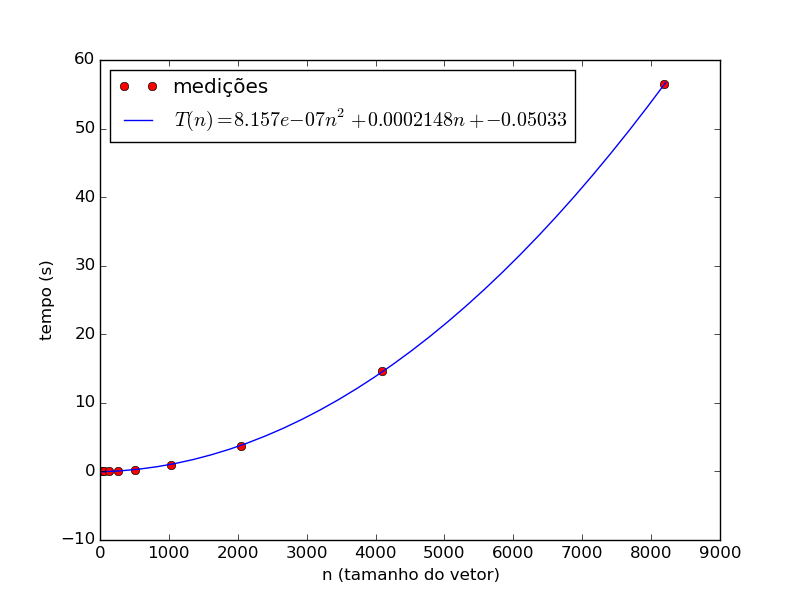
\includegraphics[scale=0.8]{../insertionsort/imagens/insertionsortQuaseDecresc100.png}
\caption{A análise do grafico para $2^{32}$ segue abaixo para insertionsort de vetor quase decrescente 10\%.\\
Tendo a função $T(n) = 8.157\mathrm{e}-07*n^2+0.0002148*n-0.05033$ e para o $n =2^{32}$, $T(2^{32}) = 1.46637829 * 10^{302}$}
\label{fig:insertionsortQuaseDecresc100}
\end{figure}

\begin{figure}[ht]
\centering 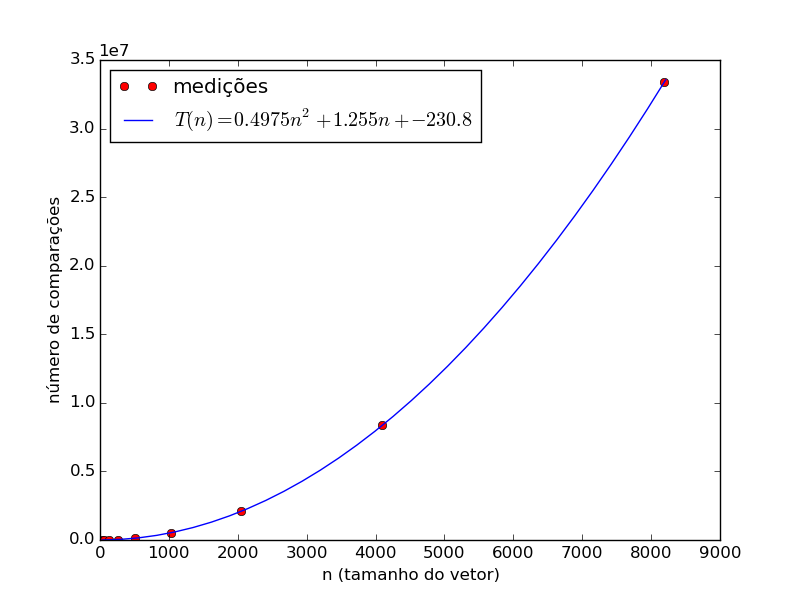
\includegraphics[scale=0.8]{../insertionsort/imagens/insertionsortQuaseDecresc101.png}
\caption{A análise do grafico para $2^{32}$ segue abaixo para insertionsort de vetor quase decrescente 10\%.\\
Tendo a função $T(n) = 0.4975*n^2+1.255*n-230.8$ e para o $n =2^{32}$, $T(2^{32}) = 8.743006299 * 10^{158}$}
\label{fig:insertionsortQuaseDecresc101}
\end{figure}


\input{../insertionsort/tabelas/insertionsortQuaseDecresc20.tex}

\begin{figure}[ht]
\centering 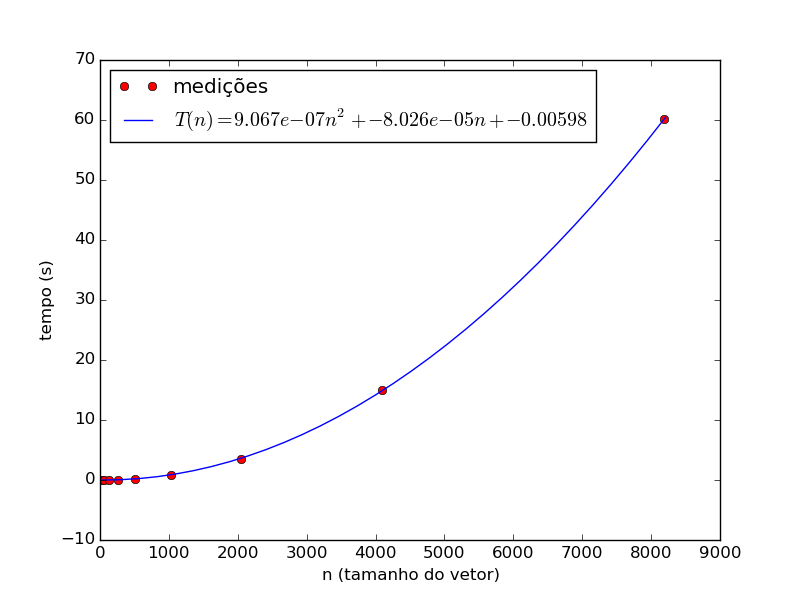
\includegraphics[scale=0.8]{../insertionsort/imagens/insertionsortQuaseDecresc200.png}
\caption{A análise do grafico para $2^{32}$ segue abaixo para insertionsort de vetor quase decrescente 20\%.\\
Tendo a função $T(n) = 9.067mathrm{e}-07*n^2+8.026\mathrm{e}-05*n-0.00598$ e para o $n =2^{32}$, $T(2^{32}) = 1.62996836 * 10^{302}$}
\label{fig:insertionsortQuaseDecresc200}
\end{figure}

\begin{figure}[ht]
\centering 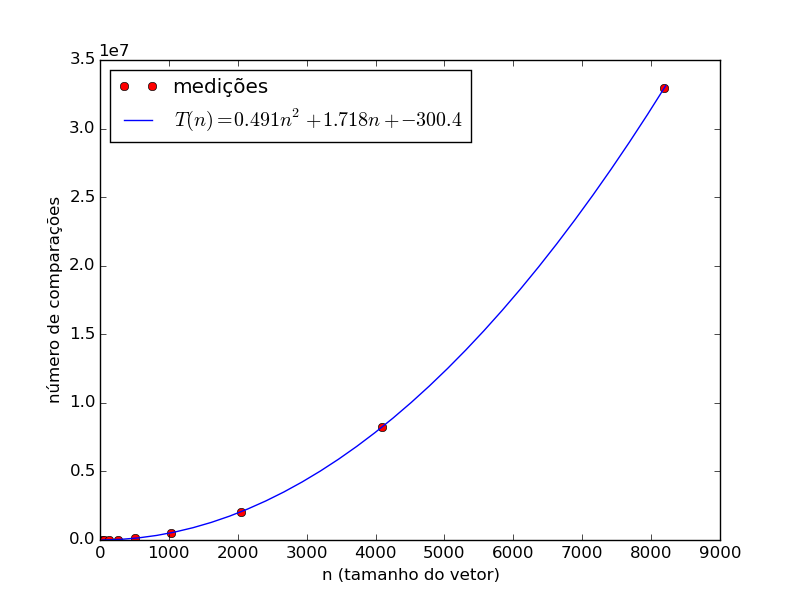
\includegraphics[scale=0.8]{../insertionsort/imagens/insertionsortQuaseDecresc201.png}
\caption{A análise do grafico para $2^{32}$ segue abaixo para insertionsort de vetor quase decrescente 20\%.\\
Tendo a função $T(n) = 0.491*n^2+1.718*n-300.4$ e para o $n =2^{32}$, $T(2^{32}) = 8.8266732921 * 10^{307}$}
\label{fig:insertionsortQuaseDecresc201}
\end{figure}

\clearpage
\input{../insertionsort/tabelas/insertionsortQuaseDecresc30.tex}

\begin{figure}[ht]
\centering 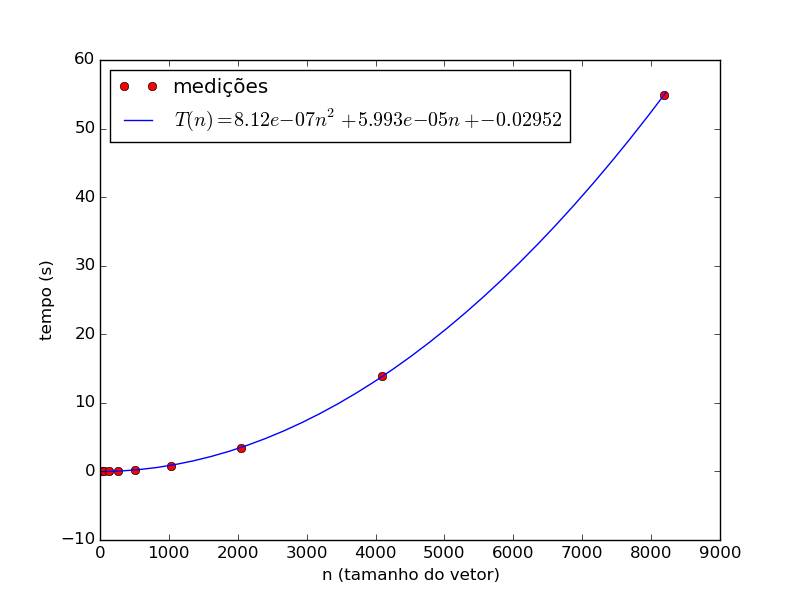
\includegraphics[scale=0.8]{../insertionsort/imagens/insertionsortQuaseDecresc300.png}
\caption{A análise do grafico para $2^{32}$ segue abaixo para insertionsort de vetor quase decrescente 30\%.\\
Tendo a função $T(n) = 8.12\mathrm{e}-07*n^2+5993\mathrm{e}-05*n-0.02952$ e para o $n =2^{32}$, $T(2^{32}) = 1.4597268 * 10^{302}$}
\label{fig:insertionsortQuaseDecresc300}
\end{figure}

\begin{figure}[ht]
\centering 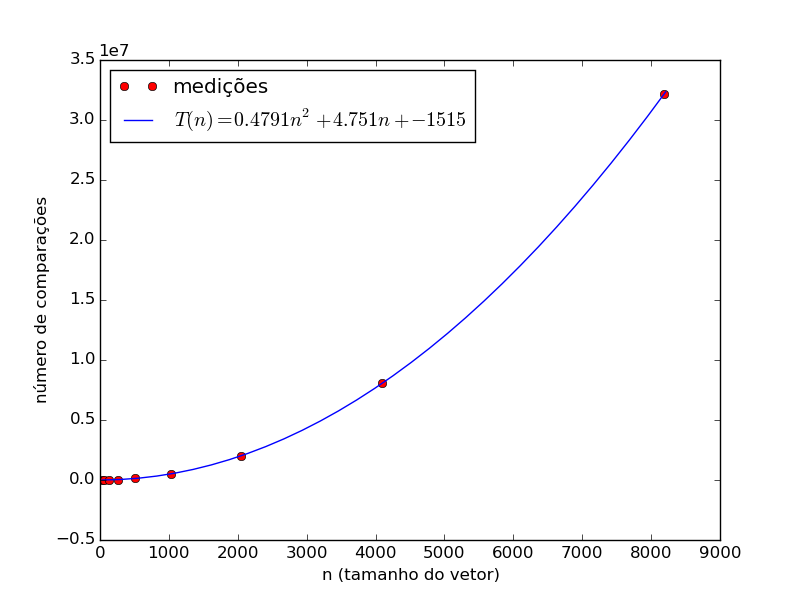
\includegraphics[scale=0.8]{../insertionsort/imagens/insertionsortQuaseDecresc301.png}
\caption{A análise do grafico para $2^{32}$ segue abaixo para insertionsort de vetor quase crescente 30\%.\\
Tendo a função $T(n) = 0.4791*n^2+4.751*n-1515$ e para o $n =2^{32}$, $T(2^{32}) = 8.6127478 * 10^{307}$}
\label{fig:insertionsortQuaseDecresc301}
\end{figure}


\input{../insertionsort/tabelas/insertionsortQuaseDecresc40.tex}

\begin{figure}[ht]
\centering 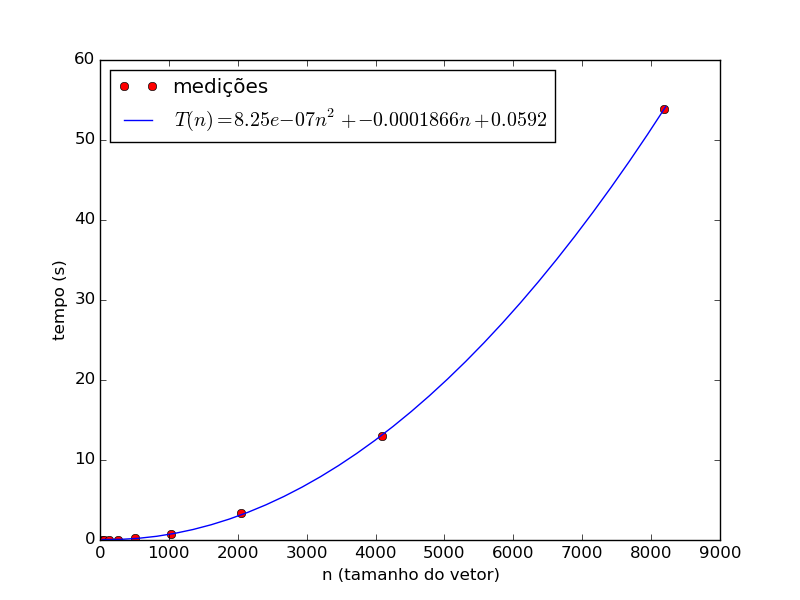
\includegraphics[scale=0.8]{../insertionsort/imagens/insertionsortQuaseDecresc400.png}
\caption{A análise do grafico para $2^{32}$ segue abaixo para insertionsort de vetor quase decrescente40 \%.\\
Tendo a função $T(n) = 8.25\mathrm{e}-07*n^2-0.0001866\mathrm{e}-05*n+0.0592$ e para o $n =2^{32}$, $T(2^{32}) = 1.4830968 * 10^{302}$}
\label{fig:insertionsortQuaseDecresc400}
\end{figure}

\begin{figure}[ht]
\centering 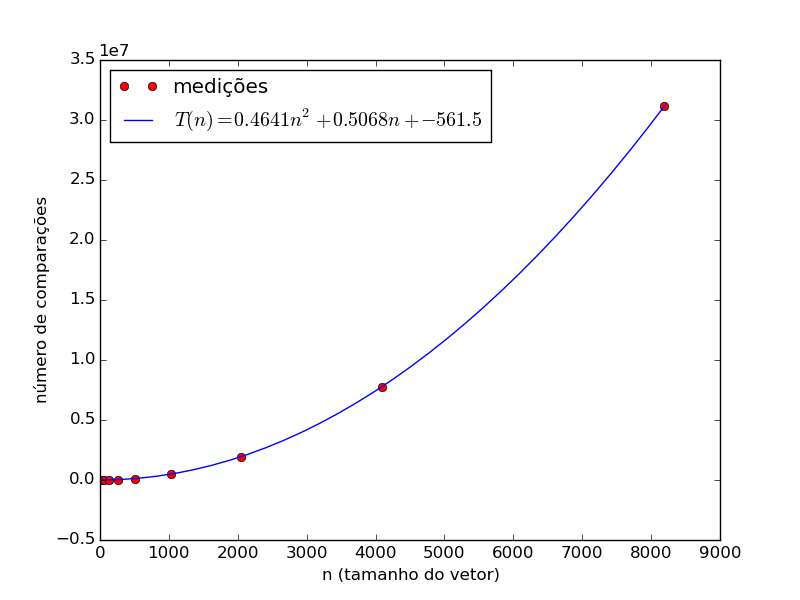
\includegraphics[scale=0.8]{../insertionsort/imagens/insertionsortQuaseDecresc401.png}
\caption{A análise do grafico para $2^{32}$ segue abaixo para insertionsort de vetor quase crescente 40\%.\\
Tendo a função $T(n) = 0.4641*n^2+0.5068*n+561.5$ e para o $n =2^{32}$, $T(2^{32}) = 8.34309383 * 10^{307}$}
\label{fig:insertionsortQuaseDecresc401}
\end{figure}


\begin{table}[ht]
\centering
\begin{tabular}{rrr} \toprule
        n &    comparações &       tempo(s) \\ \midrule
      32  &            468 &      0.000836 \\
      64  &           1855 &      0.003026 \\
     128  &           7267 &      0.011943 \\
     256  &          29123 &      0.046065 \\
     512  &         116387 &      0.194005 \\
    1024  &         468836 &      0.832933 \\
    2048  &        1863423 &      3.550210 \\
    4096  &        7458964 &     12.681700 \\
    8192  &       29758852 &     50.685500 \\
\bottomrule\addlinespace
\end{tabular}
\caption{Tabela com vetor teste quase decrescente 50\%: a linha de interesse analisada para este caso é a 15}
\label{tab:insertionsortQuaseDecresc50}
\end{table}


\begin{figure}[ht]
\centering 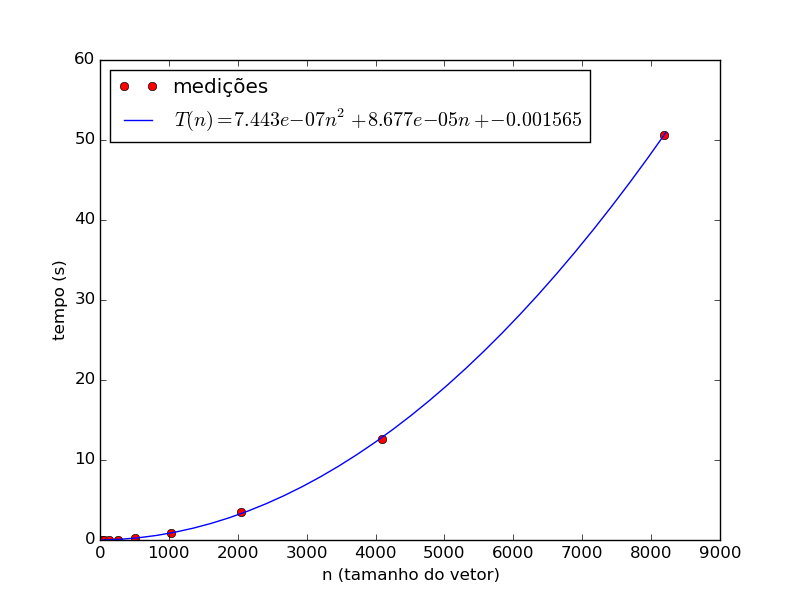
\includegraphics[scale=0.8]{../insertionsort/imagens/insertionsortQuaseDecresc500.png}
\caption{A análise do grafico para $2^{32}$ segue abaixo para insertionsort de vetor quase decrescente 50 \%.\\
Tendo a função $T (n) = 7.443\mathrm{e}-07*n^2+9.677\mathrm{e}-05*n+0.001565 $ e para o $n =2^{32}$, $T(2^{32}) = 1.3380230 * 10^{303}$}
\label{fig:insertionsortQuaseDecresc500}
\end{figure}

\begin{figure}[ht]
\centering 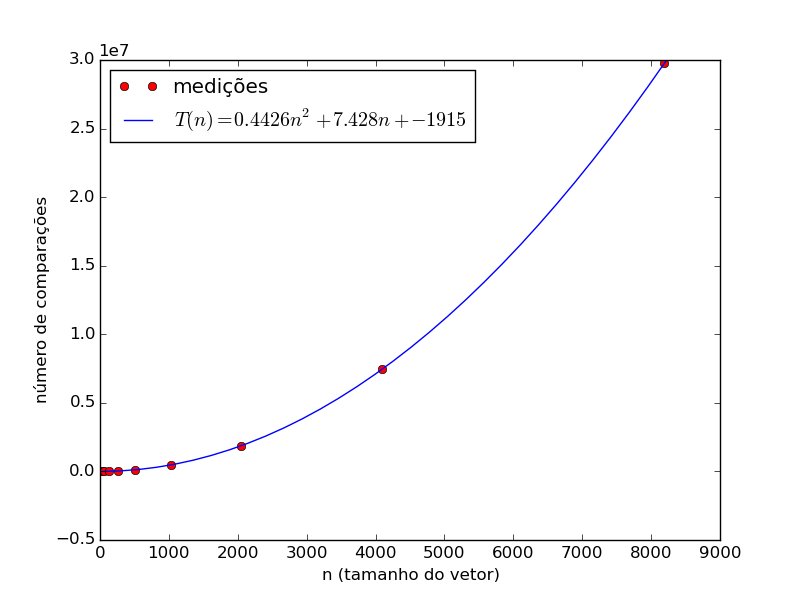
\includegraphics[scale=0.8]{../insertionsort/imagens/insertionsortQuaseDecresc501.png}
\caption{A análise do grafico para $2^{32}$ segue abaixo para insertionsort de vetor quase decrescente 50\%.\\
Tendo a função $T(n) = 0.4426*n^2+7.428*n-1915$ e para o $n =2^{32}$, $T(2^{32}) = 7.9565898 * 10^{307}$}
\label{fig:insertionsortQuaseDecresc501}
\end{figure}


\clearpage
\clearpage
\addcontentsline{toc}{part}{Apêndice}
\appendix

\chapter{Arquivo ../insertionsort/insertionsort.py \label{ap:insertionsort}}
\lstinputlisting[caption={../insertionsort/insertionsort.py \label{arq:insertionsort}}]{../insertionsort/insertionsort.py}

\chapter{Arquivo ../insertionsort/ensaio.py \label{ap:insertionsortensaio}}
\lstinputlisting[caption={../insertionsort/ensaio.py \label{arq:insertionsortensaio}}]{../insertionsort/ensaio.py}

\end{document}
